
\section{Simulation and Results}

In this section we will test the proposed DiSR approach to demonstrate
its effectiveness from two different perspectives:
\begin{itemize}
\item Against the centralized segment based approach (SR), to evaluate
if and how its known properties are still preserved in the new nano-scale distributed scenario
\item Against topology agnostic approaches based on spanning
trees and broadcasting, to measure how DiSR performs in discovering
the network structure 
\end{itemize}

\subsection{Nanoxim environment}

In order to quantitatively and qualitatively evaluate the proposed approach a
specific simulation environment has been developed, resulting in
the open source and freely available project called
Nanoxim~\cite{nanoxim}.
Nanoxim is a SystemC tool based on a almost rewritten
version of the Noxim Network-on-Chip simulator~\cite{noxim}. While some
complex features have been removed (e.g. wormhole, congestion/topology
aware routing and selection strategies) new features specifically
taylored for nanoscale scenario were introduced, e.g. the ability to simulate a random
network, the implementation of the DiSR to obtain the segment topology
and the support for defective links and nodes.

%------------------------------------------------------------------------------
\subsection{Experimental setup}
The following parameters have been taken into account when
performing the DiSR simulation:
\begin{itemize}
\item {\emph{Size of the network}}: number of nodes, on a
range from 10x10 to 100x100 sized networks. 
%\item {\% defective links}: the probability that each link is
%disconnected or not present, from 0 the amount that yelds
%no more segments.
\item {\emph{\% defective nodes}}: the probability that a node is not
working, thus having all its links cannot be utilized during DiSR setup.  
%Same range as defective links parameter.
\item {Bootstrap node}: the node used from upper layer 
to inject the DiSR process. When not explicitly investigating the
impact of each single bootstrap choice, a set representative regions have been
considered, i.e. the central part of the network and the edge corners
\end{itemize}

The show the results, the following evaluation metrics have been adopted:
\begin{itemize}
\item{Node coverage}: this is the fraction of nodes that
are assigned to a segment. In the ideal case, all the non defective
nodes should be assigned, so this metric is useful to show how some
disconnected node regions can negativaly impact on the whole DiSR
effectiveness.
\item{Broadcast latency}: this measures how the time required to complete the
segment assignment scale for increasing network sizes and defect rates
\item{Bootstrap node effect}: this evaluates the impact of the chosen
bootstrap node on the node coverage.
\end{itemize}

Further, to evaluate how DiSR compares against the centralized segment
based algorithm, the following metrics have been adopted:
\begin{itemize}
%\item {Average Path Lenght}:
%\item {Average Link Weight}:
\item {Unidirectional restrictions:}
\item {Number of Segments}:
\end{itemize}

Since the distribution of defects and thus the resulting topology is randomly
generated, a set of simulations with different seeds has been run
for each system configuration. We found that 20 repetitions are
required in order to obtain statistically significant results.

% TODO: long paper
%\subsection{Other optimisations}
%Some optimisation parameters, which demostrated to improve the DiSR
%results have been fixed to some good values, but are not subject to
%further investigation; once again the focus here is not the
%optimal set of segments, but just demostrating a working approach. 
%These are optimisations are:
%\begin{itemize}
%\item{cycle\_links}: max number of retries across the set of links of
%each node. While searching for a free link due an incoming request,
%the same request is cancelled after a given number of tries. This
%gives to preceding node change to test a different paths. Default is set to 1.
%\item{bootstrap\_timeout}: number of time units that a bootstrap node
%should wait before assuming that a livelock in the starting segment
%process has occurred. In the worst case, we can imagine that longest
%path required is the one returning to the bootstrap node after having
%travelled across all the links. So, althought this is just an extreme
%situation, a good upper limit can be safely be set to NxN.
%\item{bootstrap\_immunity}: in order to avoid the failure of the whole DiSR
%setup process, a bootstrap node should not have defective links.
%Enabling this optimisation, a bootstrap node is immune to defects.
%We may think of a pre-boostrap phase that properly selects (from upper
%layer via) a bootstrap node which is tested as properly connected. We
%enabled this optimisation, however empirical tests showed us that only
%simulations using bootstrap nodes placed on edges would be heavily
%affected, since these are nodes starting with a lower number of links,
%e.g. corner nodes could only have two connected direction, so even a
%defective link could prevent starting segment packet to return to
%bootstrap to close the loop a create the segment.
%\end{itemize}

\section{Results}
\label{sec:results}


In Figure~\ref{fig:coverage} is shown node coverage using different
network sizes and bootstrap injection points. As can be seen,
increasing the \% of defective node, TODO COMMENT... 

\begin{figure*}
  \centering
  \begin{tabular}{cc}
    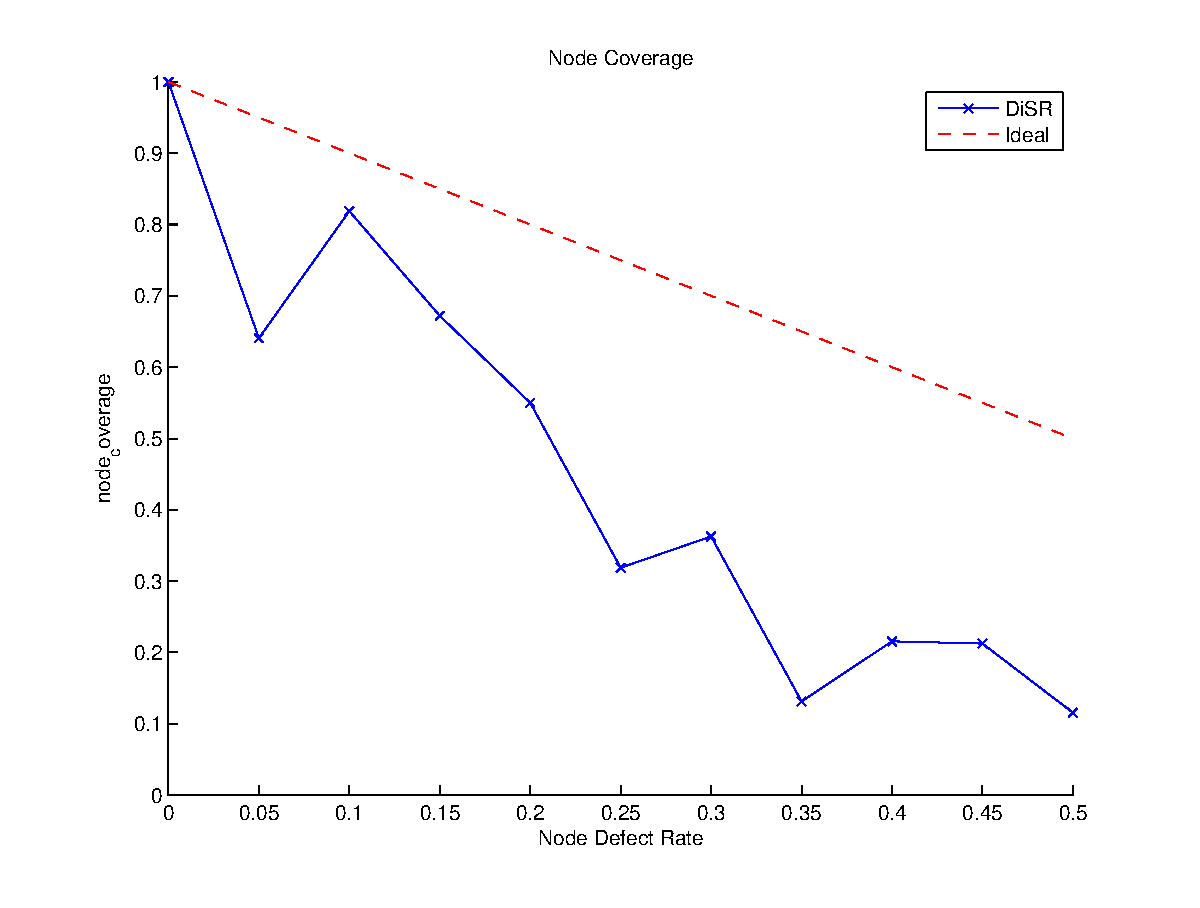
\includegraphics[width=0.40\textwidth]{pictures/set1.eps} & 
    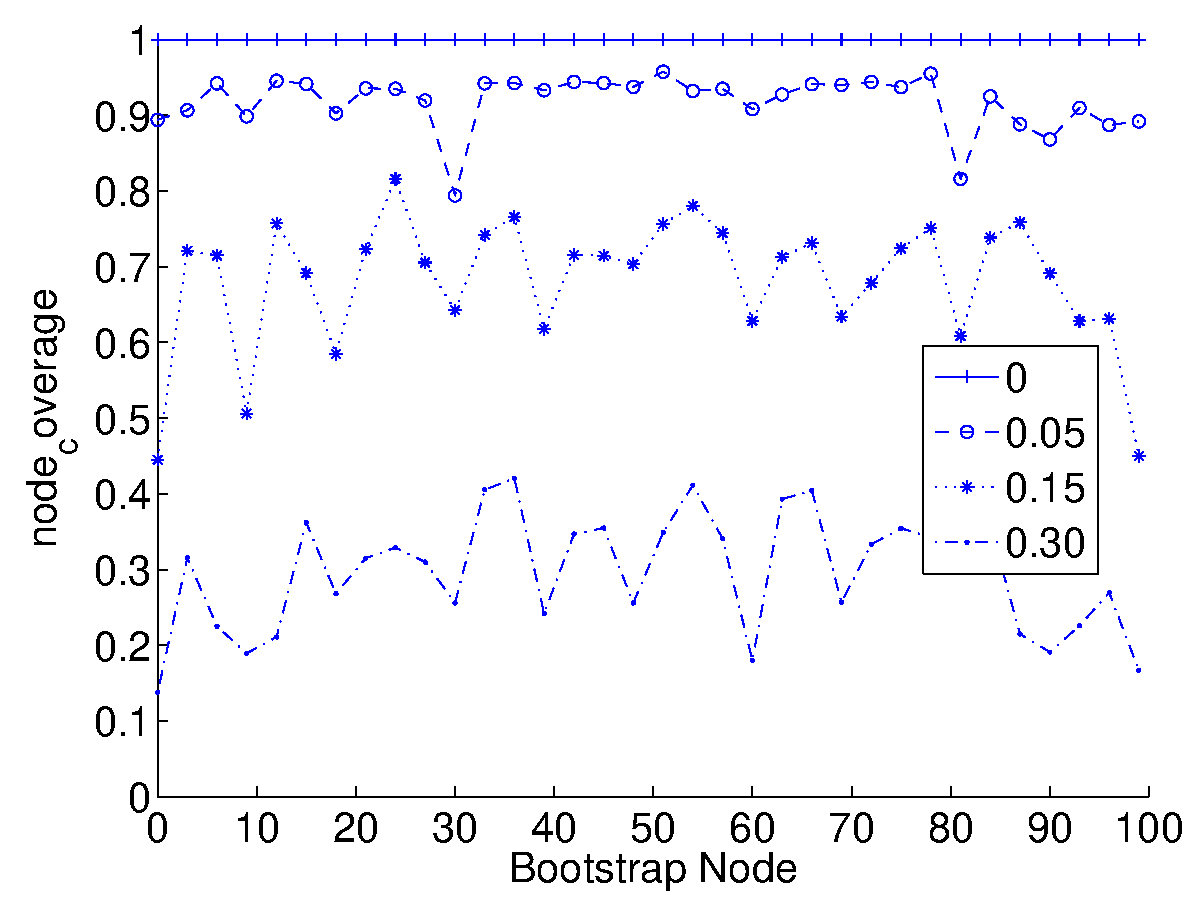
\includegraphics[width=0.40\textwidth]{pictures/set3.eps} \\
    (a) & (b)
  \end{tabular}
  \caption{Node coverage in function of Node defect rates at 8x8 (a) and 15x15 (b) network sizes}
  \label{fig:coverage}
\end{figure*}

Figure~\ref{fig:bootstrap} shows the effect of bootstrap node position
on node coverage, for different defect rates. TODO COMMENT.


%\begin{figure}
%  \centering
%  \begin{tabular}{cc}
%    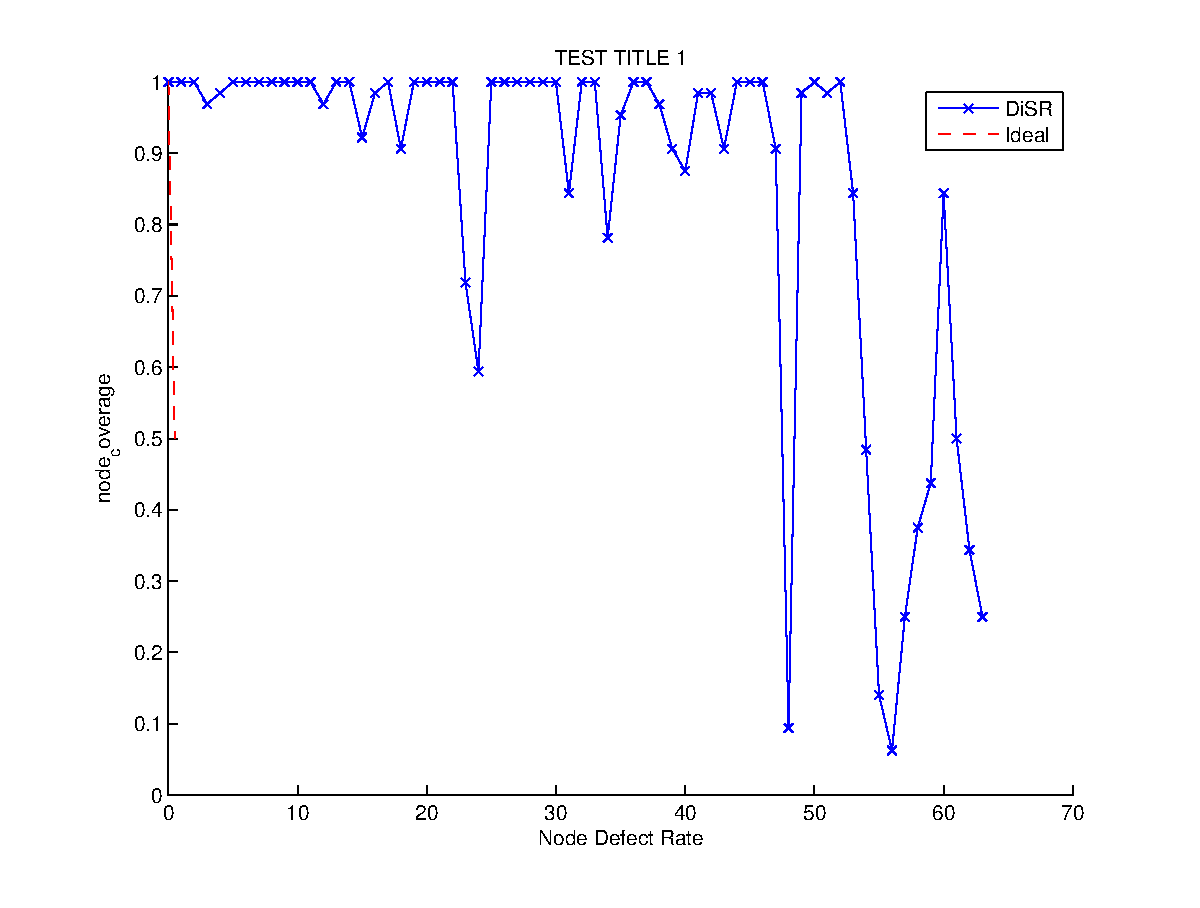
\includegraphics[width=0.40\textwidth]{pictures/sim8x8_nodefect_Xbootstrap_Ycoverage.eps} & 
%    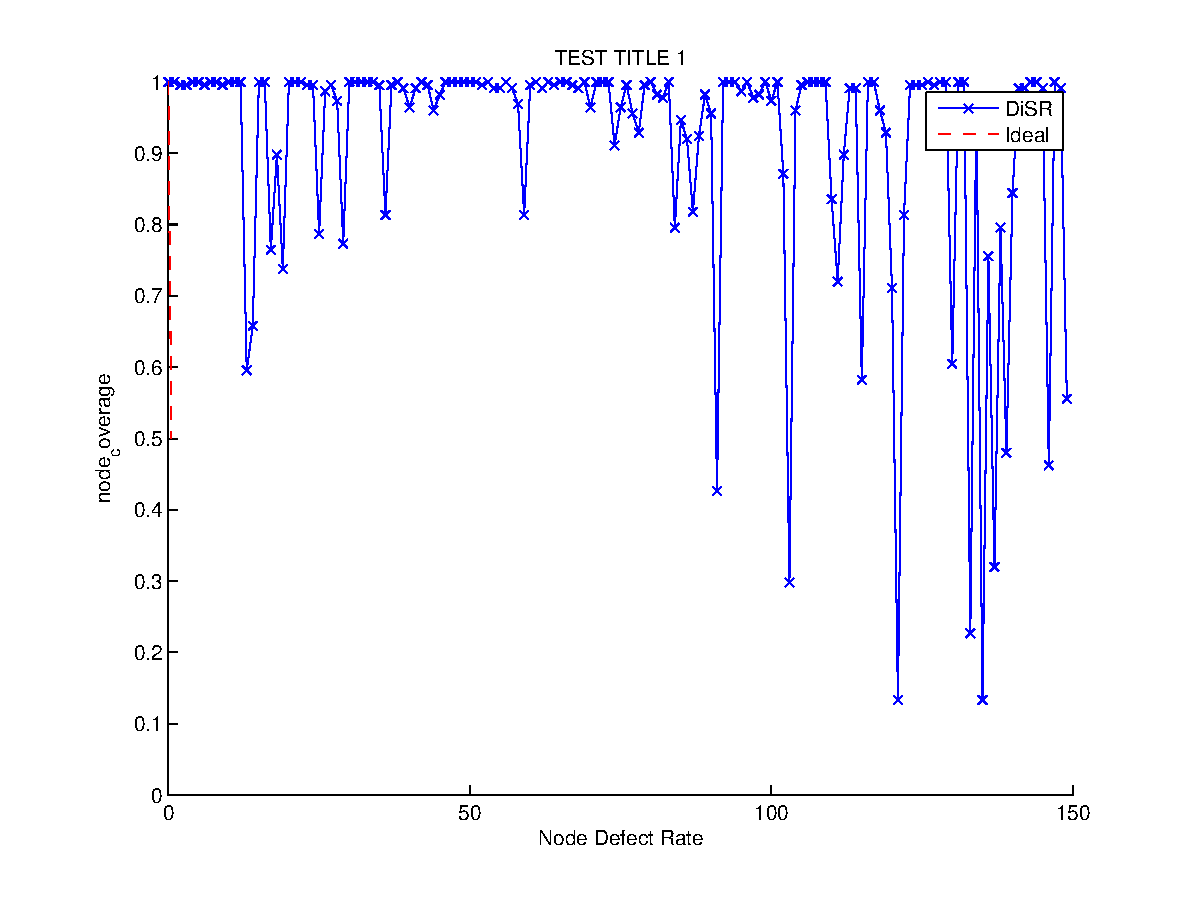
\includegraphics[width=0.40\textwidth]{pictures/sim15x15_nodefect_Xbootstrap_Ycoverage.eps} \\
%    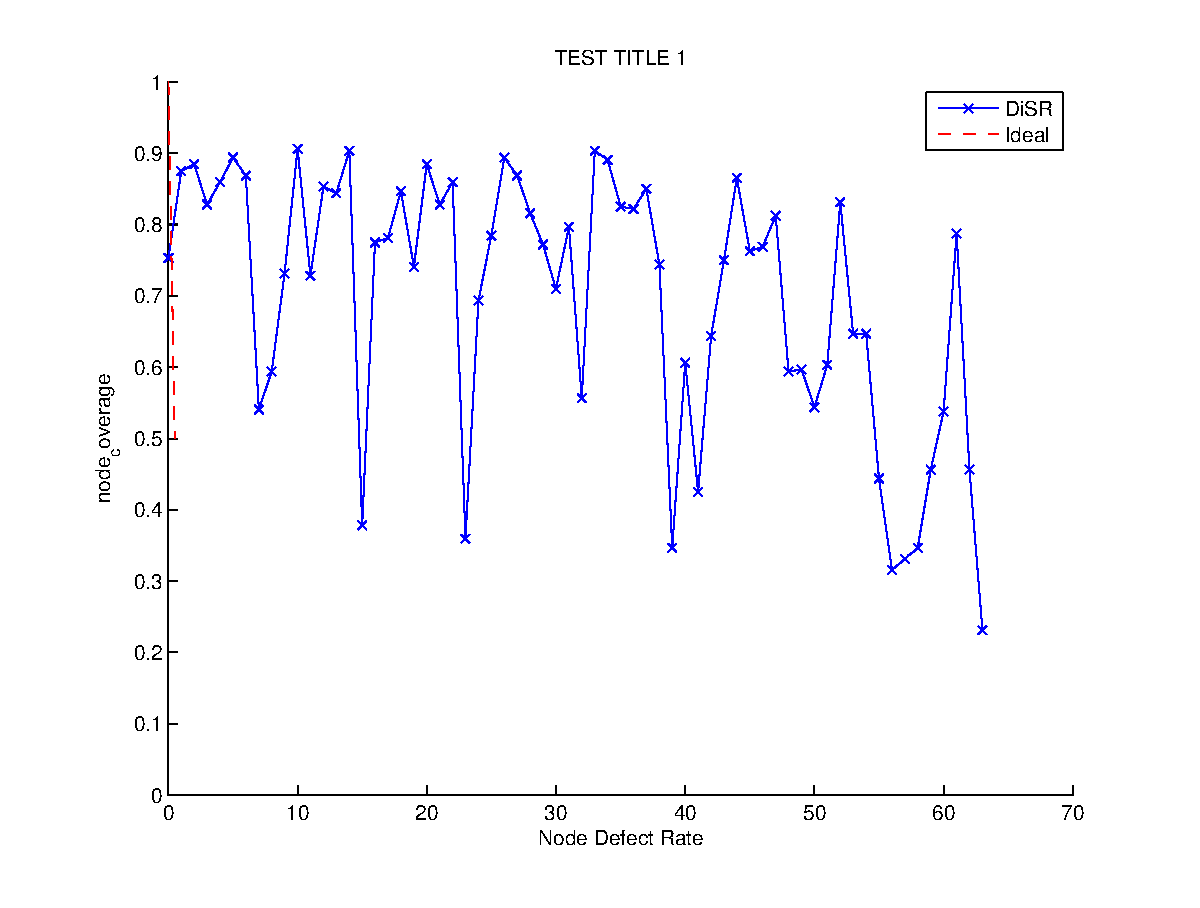
\includegraphics[width=0.40\textwidth]{pictures/sim8x8_defect01_Xbootstrap_Ycoverage.eps} & 
%    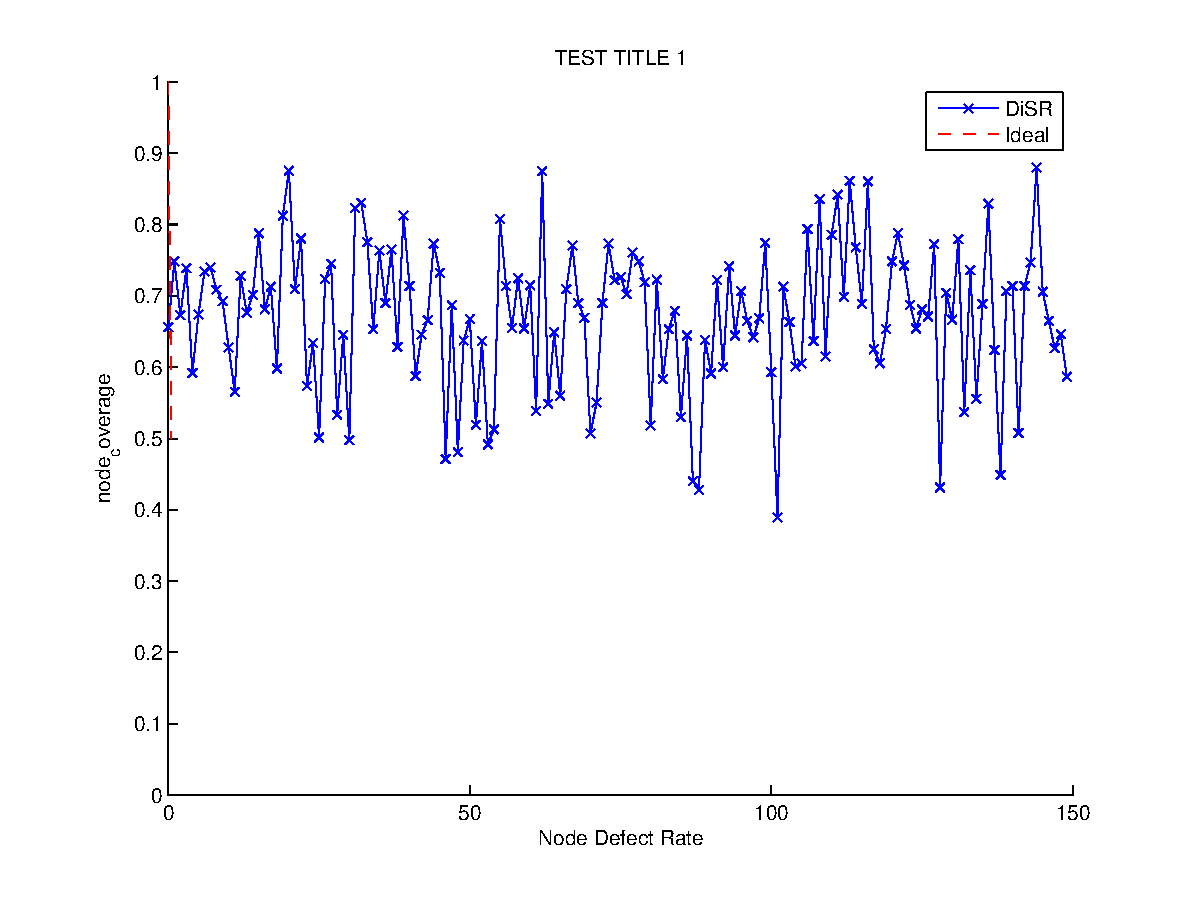
\includegraphics[width=0.40\textwidth]{pictures/sim15x15_defect01_Xbootstrap_Ycoverage.eps} \\
%    (a) & (b)
%  \end{tabular}
%  \caption{Node coverage in function of Node defect rates at 8x8 (a) and 15x15 (b) network sizes}
%  \label{fig:bootstrap}
%\end{figure}

Next, Figure~\ref{fig:latency_size} shows latency as function of
network size, with different defect rates, while Figure~\ref{fig:latency_defective}
shows the same latency when different bootstrap nodes are
considered.... TODO COMMENT

TODO: something like Broadcast Tree properties (sez.  5.4)

